\hypertarget{group__park}{}\section{Vector Park Transform}
\label{group__park}\index{Vector Park Transform@{Vector Park Transform}}
Collaboration diagram for Vector Park Transform\+:
\nopagebreak
\begin{figure}[H]
\begin{center}
\leavevmode
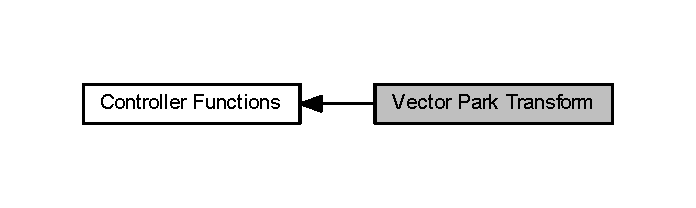
\includegraphics[width=334pt]{group__park}
\end{center}
\end{figure}


\subsection{Detailed Description}
Forward Park transform converts the input two-\/coordinate vector to flux and torque components. The Park transform can be used to realize the transformation of the {\ttfamily Ialpha} and the {\ttfamily Ibeta} currents from the stationary to the moving reference frame and control the spatial relationship between the stator vector current and rotor flux vector. If we consider the d axis aligned with the rotor flux, the diagram below shows the current vector and the relationship from the two reference frames\+:  The function operates on a single sample of data and each call to the function returns the processed output. The library provides separate functions for Q31 and floating-\/point data types. \begin{DoxyParagraph}{Algorithm}
 where {\ttfamily Ialpha} and {\ttfamily Ibeta} are the stator vector components, {\ttfamily p\+Id} and {\ttfamily p\+Iq} are rotor vector components and {\ttfamily cos\+Val} and {\ttfamily sin\+Val} are the cosine and sine values of theta (rotor flux position). 
\end{DoxyParagraph}
\begin{DoxyParagraph}{Fixed-\/\+Point Behavior}
Care must be taken when using the Q31 version of the Park transform. In particular, the overflow and saturation behavior of the accumulator used must be considered. Refer to the function specific documentation below for usage guidelines. 
\end{DoxyParagraph}
